\chapter{Modello Fisico e Ottimizzazione}

\section*{Introduzione}
Il modello fisico descrive come i dati sono effettivamente memorizzati e organizzati nel disco fisico. Include indici, viste materializzate, partizionamento e altre strategie di ottimizzazione per migliorare performance e scalabilità.

\section*{Obiettivi di apprendimento}
\begin{itemize}
    \item Comprendere come i dati sono memorizzati nel disco
    \item Progettare e utilizzare indici efficaci
    \item Comprendere le viste materializzate e il caching
    \item Applicare strategie di partizionamento
    \item Ottimizzare query e accessi ai dati
    \item Bilanciare velocità di lettura e velocità di scrittura
\end{itemize}

\section{Memorizzazione dei Dati}

\subsection{Struttura di memorizzazione}
I dati vengono memorizzati in blocchi (pagine) sul disco:
\begin{itemize}
    \item \textbf{Blocco}: unità minima di trasferimento tra disco e memoria (tipicamente 4-16 KB)
    \item \textbf{Pagina}: blocco logico del DBMS
    \item \textbf{Record}: singola tupla della tabella
    \item \textbf{Campo}: singolo attributo di un record
\end{itemize}

\begin{figure}[h]
    \centering
    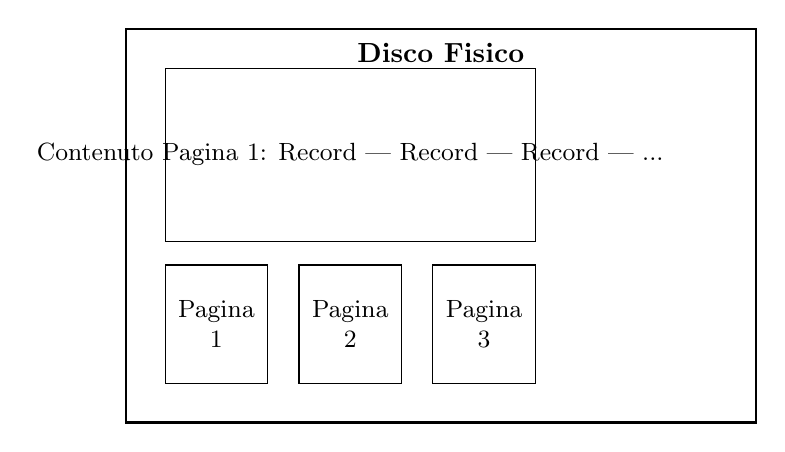
\begin{tikzpicture}[scale=1]
        \draw[thick] (0, 0) rectangle (8, 5);
        \node at (4, 4.7) {\textbf{Disco Fisico}};

        \draw (0.5, 0.5) rectangle (1.8, 2);
        \node[align=center, font=\small] at (1.15, 1.25) {Pagina\\1};

        \draw (2.2, 0.5) rectangle (3.5, 2);
        \node[align=center, font=\small] at (2.85, 1.25) {Pagina\\2};

        \draw (3.9, 0.5) rectangle (5.2, 2);
        \node[align=center, font=\small] at (4.55, 1.25) {Pagina\\3};

        \draw (0.5, 2.3) rectangle (5.2, 4.5);
        \node[align=center, font=\small] at (2.85, 3.4) {Contenuto Pagina 1: Record | Record | Record | ...};
    \end{tikzpicture}
    \caption{Struttura di memorizzazione su disco}
\end{figure}

\subsection{Tipi di accesso}
\begin{description}
    \item[\textbf{Sequential access}]: Leggere i record uno dopo l'altro sequenzialmente. Lento per record specifici.
    \item[\textbf{Random access}]: Accedere direttamente a un record senza leggerne altri. Veloce ma necessita di indici.
\end{description}

\section{Indici}

Un \textbf{indice} è una struttura dati che accelera il recupero di record da una tabella. Funziona come un indice di un libro: invece di leggere tutte le pagine, consulti l'indice per trovare la pagina che cerchi.

\subsection{Vantaggi degli indici}
\begin{itemize}
    \item Accelera ricerche e filtri (WHERE)
    \item Accelera ordinamenti (ORDER BY)
    \item Accelera join tra tabelle
    \item Supporta query range (es. WHERE prezzo BETWEEN 10 AND 100)
\end{itemize}

\subsection{Svantaggi degli indici}
\begin{itemize}
    \item Occupano spazio aggiuntivo su disco
    \item Ralentano INSERT, UPDATE, DELETE (l'indice deve essere aggiornato)
    \item Richiedono manutenzione periodica
\end{itemize}

\subsection{Tipi di indici}

\subsubsection{Indice primario}
Un indice su una chiave primaria. È automaticamente creato quando si definisce una PRIMARY KEY.

\begin{lstlisting}[language=SQL, caption=Indice primario (creato automaticamente)]
CREATE TABLE cliente (
    idCliente INT PRIMARY KEY,  -- Indice primario automatico
    nome VARCHAR(100)
);
\end{lstlisting}

\subsubsection{Indice secondario}
Un indice su attributi non-chiave per accelerare ricerche frequenti.

\begin{lstlisting}[language=SQL, caption=Creare un indice secondario]
CREATE TABLE cliente (
    idCliente INT PRIMARY KEY,
    nome VARCHAR(100),
    email VARCHAR(100),
    città VARCHAR(50)
);

-- Indici su campi frequentemente cercati
CREATE INDEX idx_email ON cliente(email);
CREATE INDEX idx_città ON cliente(città);
\end{lstlisting}

\subsubsection{Indice composito}
Un indice su più attributi, utile per query che filtrano su più colonne.

\begin{lstlisting}[language=SQL, caption=Indice composito]
CREATE TABLE ordine (
    idOrdine INT PRIMARY KEY,
    dataOrdine DATE,
    idCliente INT,
    stato VARCHAR(20)
);

-- Indice su due colonne per query come:
-- WHERE idCliente = 5 AND stato = 'Spedito'
CREATE INDEX idx_cliente_stato ON ordine(idCliente, stato);
\end{lstlisting}

\subsubsection{Indice a hash}
Usa una funzione hash per mappare i valori agli indirizzi di memoria. Veloce per uguaglianza, non per range.

\subsubsection{Indice B-Tree}
La struttura più comune. Ordinato, efficiente per range e ordinamenti. Bilanciato automaticamente.

\begin{lstlisting}[language=SQL, caption=Statistiche dell'indice (MySQL)]
-- Mostra dettagli degli indici di una tabella
SHOW INDEX FROM cliente;

-- Analizza l'efficienza dell'indice
EXPLAIN SELECT * FROM cliente WHERE email = 'mario@email.com';
\end{lstlisting}

\subsection{Strategie di indicizzazione}

\begin{tcolorbox}[colback=green!10, colframe=green!60, title=Buone pratiche per gli indici]
\begin{itemize}
    \item Indicizza campi usati frequentemente in WHERE, JOIN, ORDER BY
    \item Non indicizzare campi usati raramente (spreco di spazio)
    \item Indici compositi per query multi-colonna frequenti
    \item Evita indici su colonne con pochi valori distinti (low cardinality)
    \item Monitora e mantieni gli indici regolarmente
\end{itemize}
\end{tcolorbox}

\section{Viste Materializzate}

Una \textbf{vista materializzata} è il risultato di una query pre-calcolato e memorizzato fisicamente sul disco. A differenza di una vista normale, occupa spazio e deve essere aggiornato.

\subsection{Vantaggi}
\begin{itemize}
    \item Query molto veloce (dati pre-calcolati)
    \item Riduce carico computazionale
    \item Utile per query complesse su dati storici
\end{itemize}

\subsection{Svantaggi}
\begin{itemize}
    \item Occupa spazio su disco
    \item Deve essere aggiornato periodicamente
    \item Dati possono essere non aggiornati (stali)
\end{itemize}

\subsection{Esempio di vista materializzata}

\begin{lstlisting}[language=SQL, caption=Vista materializzata]
-- Vista normale (calcolata ogni volta)
CREATE VIEW vendite_mensili AS
    SELECT
        MONTH(dataOrdine) AS mese,
        YEAR(dataOrdine) AS anno,
        SUM(totale) AS ricavi,
        COUNT(*) AS numOrdini
    FROM ordine
    GROUP BY YEAR(dataOrdine), MONTH(dataOrdine);

-- In MySQL, simula una vista materializzata con tabella
CREATE TABLE vendite_mensili_cache (
    mese INT,
    anno INT,
    ricavi DECIMAL(12, 2),
    numOrdini INT,
    dataAggiornamento TIMESTAMP
) AS
SELECT
    MONTH(dataOrdine) AS mese,
    YEAR(dataOrdine) AS anno,
    SUM(totale) AS ricavi,
    COUNT(*) AS numOrdini
FROM ordine
GROUP BY YEAR(dataOrdine), MONTH(dataOrdine);

-- Aggiorna periodicamente (es. ogni notte)
-- DELETE FROM vendite_mensili_cache;
-- INSERT INTO vendite_mensili_cache (SELECT ...);
\end{lstlisting}

\section{Partizionamento}

Il \textbf{partizionamento} divide una tabella grande in parti più piccole (partizioni) basate su criteri specifici, migliorando performance e manutenzione.

\subsection{Tipi di partizionamento}

\subsubsection{Partizionamento per range}
Divide i dati in base a intervalli di valori.

\begin{lstlisting}[language=SQL, caption=Partizionamento per range (anno)]
CREATE TABLE ordine (
    idOrdine INT,
    dataOrdine DATE,
    totale DECIMAL(10, 2)
)
PARTITION BY RANGE (YEAR(dataOrdine)) (
    PARTITION p2020 VALUES LESS THAN (2021),
    PARTITION p2021 VALUES LESS THAN (2022),
    PARTITION p2022 VALUES LESS THAN (2023),
    PARTITION p2023 VALUES LESS THAN (2024),
    PARTITION pmax VALUES LESS THAN MAXVALUE
);
\end{lstlisting}

\subsubsection{Partizionamento per list}
Divide i dati in base a valori specifici.

\begin{lstlisting}[language=SQL, caption=Partizionamento per list]
CREATE TABLE ordine (
    idOrdine INT,
    stato VARCHAR(20),
    totale DECIMAL(10, 2)
)
PARTITION BY LIST (stato) (
    PARTITION p_pending VALUES IN ('Pendente'),
    PARTITION p_shipped VALUES IN ('Spedito'),
    PARTITION p_delivered VALUES IN ('Consegnato'),
    PARTITION p_other VALUES IN (DEFAULT)
);
\end{lstlisting}

\subsubsection{Partizionamento per hash}
Distribuisce i dati in base a una funzione hash.

\begin{lstlisting}[language=SQL, caption=Partizionamento per hash]
CREATE TABLE ordine (
    idOrdine INT,
    idCliente INT,
    totale DECIMAL(10, 2)
)
PARTITION BY HASH(idCliente)
PARTITIONS 4;  -- 4 partizioni
\end{lstlisting}

\subsection{Vantaggi del partizionamento}
\begin{itemize}
    \item Query più veloci (scansione solo partizioni rilevanti)
    \item Manutenzione più agevole (backup per partizione)
    \item Scalabilità orizzontale
\end{itemize}

\section{Ottimizzazione di Query}

\subsection{Utilizzo di EXPLAIN}
Il comando EXPLAIN analizza il piano di esecuzione di una query.

\begin{lstlisting}[language=SQL, caption=Analizzare il piano di esecuzione]
EXPLAIN SELECT *
FROM ordine o
JOIN cliente c ON o.idCliente = c.idCliente
WHERE c.città = 'Milano'
ORDER BY o.dataOrdine DESC;
\end{lstlisting}

L'output mostra:
\begin{itemize}
    \item Quale indice viene usato
    \item Quante righe vengono esaminate
    \item Il costo relativo di ogni operazione
\end{itemize}

\subsection{Statistiche e manutenzione}

\begin{lstlisting}[language=SQL, caption=Manutenzione degli indici]
-- Ricalcola statistiche tabella
ANALYZE TABLE ordine;

-- Ottimizza spazio tabella
OPTIMIZE TABLE ordine;

-- Mostra statistiche tabella
SHOW TABLE STATUS FROM database_name;
\end{lstlisting}

\section*{Riepilogo concetti chiave}

\begin{tcolorbox}[colback=gray!10, colframe=black!60, title=Concetti fondamentali]
\begin{itemize}
    \item I dati sono memorizzati in \textbf{pagine/blocchi} sul disco
    \item Gli \textbf{indici} accelerano ricerche, JOIN e ordinamenti
    \item Le \textbf{viste materializzate} pre-calcolano risultati frequenti
    \item Il \textbf{partizionamento} divide grandi tabelle in parti più piccole
    \item Bilanciare velocità di lettura (indici) con velocità di scrittura
    \item Monitorare con EXPLAIN e statistiche per identificare colli di bottiglia
\end{itemize}
\end{tcolorbox}

\section*{Esercizi}

\begin{enumerate}
    \item Progetta una strategia di indicizzazione per una tabella con milioni di ordini. Quali campi indicizzaresti? Perché?

    \item Una query SELECT * FROM cliente WHERE città = 'Roma' AND età > 30 è lenta. Come potrebbe aiutare un indice composito?

    \item Qual è la differenza tra una vista normal e una vista materializzata? Quando useresti ciascuna?

    \item Proponi un partizionamento per una tabella logs con milioni di record inseriti ogni giorno.

    \item Analizza il seguente piano di esecuzione e proponi ottimizzazioni:
    \begin{lstlisting}[language=SQL]
EXPLAIN SELECT *
FROM ordine
WHERE dataOrdine > '2023-01-01' AND stato = 'Spedito';
    \end{lstlisting}

    \item Crea una vista materializzata per memorizzare le vendite totali per cliente nel 2023. Come la aggiornare settimanalmente?
\end{enumerate}
